\chapter{Monopole design}

A monopole antenna is the most simple antenna, as it is a wire, where the signal generator is connected at one end and nothing a the other end. It is normally place atop of a ground plane. The radiation pattern is the same as a dipole antenna with a larger ground plane, which is a doughnut shape, where there is less to none radiation directly above and below the antenna, while the strength of the radiation gets better, the more horizontal the direction gets. But if the ground plane is not large enough, the doughnut shape, will be tilted more upwards.

\begin{figure}[H]
\centering
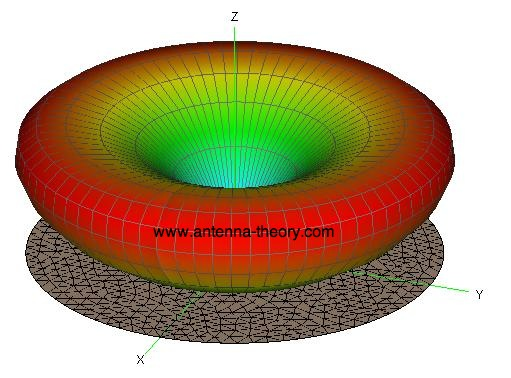
\includegraphics[width=0.5\textwidth]{figure/disturbedMonopole.jpg}
\caption{Radiation pattern of a quarter length monopole antenna, with a ground plane with a diameter on 3 wavelength.}
\label{fig:disMono}
\end{figure}

The frequency of the monopole antenna is determined by the length of the antenna, like the dipole antenna. The antenna needs a length equal to a forth of the wavelength of the wanted frequency, which is equal to half the size of a dipole antenna, with same frequency. With this length, it will have a input impedances on $(36.5 + 21.25j) \ohm$.

\begin{equation}\label{eq:lengthMono}
L = \frac{\lambda}{4}
\end{equation}
\begin{where}
\va{$L$}{is the length of the antenna}{m}
\va{$\lambda$}{is the wavelength of the wanted frequency}{m}
\end{where}

